% Данный файл распространяется под лицензией CC BY 4.0. Текст лицензии размещён на https://creativecommons.org/licenses/by/4.0/
% (c) Кафедра системного программирования, 2026

% Компилировать XeTeX

\documentclass[a4paper]{article}

\usepackage[a4paper, top=8mm, bottom=8mm, left=8mm, right=8mm]{geometry}

\usepackage{polyglossia}
\setdefaultlanguage[babelshorthands=true]{russian}
\setotherlanguage{english}

\usepackage{fontspec}
\setmainfont{FreeSerif}
\newfontfamily{\russianfonttt}[Scale=0.7]{DejaVuSansMono}

\usepackage[tiny, compact]{titlesec}

\usepackage{titling}
\setlength{\droptitle}{-1cm}
\pretitle{\begin{center}\begin{bfseries}\Large}
\posttitle{\par\end{bfseries}\end{center}}
\preauthor{\begin{center}\normalsize}
\postauthor{\par\end{center}\vspace{-1.8cm}}

\usepackage{hyperref}
\usepackage{bookmark}
\usepackage{csquotes}
\usepackage{booktabs}
\usepackage{multirow}
\usepackage{graphicx}
\usepackage{float} 
% Сюда можно дописывать нужные вам пакеты.

\title{Архиватор на базе алгоритма Хаффмана}

\author{Разгуляева Ада Игоревна}

% Дата много места занимает, её лучше не указывать.
\date{}

\begin{document}

\maketitle

\begin{flushright}
    Группа: \emph{25.Б42-мм}

    Кафедра: \emph{системного программирования}

    % Степень/звание и должность научника мы лучше вас знаем, их можно не указывать.
    Научный руководитель: \emph{Литвинов Юрий Викторович}

    % А вот про консультанта укажите официальное место работы, с "ООО" или чем-то таким, и должностью желательно по трудовой, не просто "techlead". Выясните у консультанта.
    % Если консультанта нет (а на первом курсе у вас скорее всего его нет), просто удалите это.
    
    Номер семестра практики: \emph{2}
\end{flushright} 

\section{Введение}

Данная работа выполнена в рамках учебной практики. Алгоритм Хаффмана — классический метод сжатия данных без потерь, основанный на построении префиксных кодов переменной длины [1]. Код каждого символа строится так, что ни один код не является префиксом другого, что позволяет однозначно восстанавливать исходные данные. Реализация требует работы с битовыми операциями, динамическими структурами данных и бинарными файлами, что делает её полезной для освоения низкоуровневых возможностей языка C.

% \textbf{Требуемый размер всего текста практики~--- три страницы}, так что не увлекайтесь. Учитесь писать максимально сжато, чётко, по сути и с фактами~--- в эпоху больших языковых моделей полотна текста и красивый литературный стиль ценности не имеют.

\section{Постановка задачи}

\textbf{Целью работы является} получение практического опыта низкоуровневой 
разработки путём создания консольного приложения на C, выполняющего сжатие и разжатие
файлов по алгоритму Хаффмана и экспериментальная оценка его эффективности.

\textbf{Для достижения цели требуется решить следующие задачи:}
\begin{enumerate}
    \item Выполнить обзор существующих реализаций алгоритма Хаффмана.
    \item Спроектировать архитектуру консольного приложения.
    \item Реализовать консольное приложение.
    \item Выполнить тестирование и экспериментальное исследование.
\end{enumerate}

\section{Обзор}

\subsection{Основные понятия}

\textbf{Префиксный код} — способ кодирования, при котором ни один код
символа не является началом (префиксом) другого. Благодаря этому
сообщение декодируется однозначно, без разделителей между кодами.
Например, если код буквы «а» равен~\texttt{0}, то ни один другой
символ не может иметь код, начинающийся с~\texttt{0}.

\textbf{Код Хаффмана} — оптимальный префиксный код, в котором
часто встречающиеся символы получают короткие кодовые слова,
а редкие~--- длинные. Строится по частотам символов: два самых
редких символа объединяются в узел с суммарной частотой, и так
до тех пор, пока не останется один корневой узел. Длина кода
символа равна глубине соответствующего листа в дереве [1].

\textbf{Энтропия} источника — теоретический предел сжатия,
вычисляемый по распределению частот символов. Ни один префиксный
код не может дать среднюю длину кода меньше энтропии, поэтому
её значение показывает, насколько хорошо в принципе сжимаются
данные.

\textbf{Канонические коды} — разновидность кодов Хаффмана,
в которой кодовые слова для заданных длин строятся по единому
правилу (сортировка по длине и значению символа). Это позволяет
хранить в заголовке только длины кодов, а не сами коды, что
уменьшает размер служебной информации. В данной работе
используется классический код Хаффмана без канонизации.

\subsection{Обзор реализаций}

В качестве ориентиров рассмотрены открытые реализации на языке C:

\begin{itemize}
    \item SmnTin/huffman-archiver [2]: архиватор с каноническими кодами Хаффмана, оптимизированный для больших файлов.
    \item MichaelDipperstein/huffman [3]: простая и читаемая реализация, включающая как классические, так и канонические коды Хаффмана.
    \item ConnorDye/C-Zip [4]: учебный проект с модульной архитектурой.
\end{itemize}

\textbf{Вывод из обзора.} Анализ существующих реализаций [2–4] позволил выделить общие архитектурные решения. 
Из C-Zip [4] заимствована модульная структура: битовый I/O, очередь с приоритетами и дерево Хаффмана 
разделены по функциям внутри модуля. Подход к буферизованной побитовой записи и сериализации таблицы кодов в заголовок, 
встречающийся в ряде рассмотренных реализаций, обобщён и применён в данной работе.
Из huffman-archiver SmnTin [2] — идея буферизации вывода для ускорения работы с битами.

\section{Описание предлагаемого решения}

\subsection{Архитектура}

Проект состоит из:

\begin{itemize}
    \item src/huffman.h / src/huffman.c — публичный интерфейс и реализация (дерево, куча, битовый I/O, сжатие, распаковка);
    \item src/main.c — интерфейс командной строки.
\end{itemize}

Модуль \texttt{huffman.c} реализует одну задачу~--- сжатие
и восстановление файлов по алгоритму Хаффмана. Все внутренние
функции (\texttt{heapPush}, \texttt{bitWriterWriteBit},
\texttt{buildTreeFromFreqs} и~т.~д.) объединены общей
ответственностью и не имеют смысла вне контекста алгоритма.
Разделение на отдельные модули потребовало бы либо экспортировать
внутренние типы (\texttt{Node}, \texttt{MinHeap}), нарушая
инкапсуляцию, либо дублировать интерфейсы через функции доступа.
Публичный интерфейс вынесен в~\texttt{huffman.h}~--- это
классическое разделение интерфейса и реализации. Один модуль
также даёт компилятору больше возможностей для инлайнинга
и оптимизации, что важно для битовых операций, вызываемых
в горячем цикле. Такой подход согласуется с практикой
header-only-библиотек в C (\texttt{stb}, \texttt{sqlite3},
\texttt{sokol}).

\subsection{Технологии}

\begin{itemize}
    \item Язык C99, компилятор GCC 13 (также собирается Clang и MSVC).
    \item Система сборки: CMake ≥ 3.28.
    \item Статические анализаторы: clang-format (WebKit), clang-tidy.
    \item CI через GitHub Actions: сборка, проверка форматирования, линтинг и тесты на Linux и Windows.
\end{itemize}

\subsection{Технические детали}

\begin{itemize}
    \item Используется разрежённый заголовок (HdrSparse): записываются только ненулевые частоты.
    Это снижает накладные расходы с ~2 КБ до десятков–сотен байт для данных с небольшим
    алфавитом, таких как~текст или исходный код.
    \item Для построения дерева используется очередь с приоритетами с операциями за $O(\log n)$ вместо $O(n)$.
    \item Битовый поток упаковывается в байты с буферизацией, неполный байт сбрасывается при завершении.
    \item Отдельно обрабатывается случай одного уникального символа.
    \item Используется формат чисел little-endian, для обеспечения единого формата файла независимо от архитектуры.
\end{itemize}

\section{Эксперименты}

% Название секции можно поменять на более подходящее вашей работе

Для оценки эффективности алгоритма и анализа работы программы были
поставлены эксперименты, демонстрирующие степень сжатия, время сжатия
и время разжатия в зависимости от размера и типа входных данных.
Было протестировано шесть категорий данных: сильно повторяющиеся
(repeated, .bin), текстовые (text, .txt), исходный код (code, .c),
случайные байты (random, .bin), уже сжатые архивы (archive, .zip)
и изображения в формате JPEG (photo, .jpg). Размеры варьировались
от 1 КБ до 5 МБ. Для каждого файла выполнялось 10 прогонов
с расчётом математического ожидания ($\mu$) и среднеквадратичного
отклонения ($\sigma$) времени выполнения.

Эксперименты проводились на системе со следующими характеристиками:

\begin{itemize}
    \item Компилятор: gcc версии 13.3.0
    \item Флаги компиляции: -O3 -DNDEBUG (Release)
    \item Процессор: 13th Gen Intel Core i5-1335U, тактовая частота 0,4--4,6 ГГц
    \item Оперативная память: 15 ГиБ
    \item Операционная система: Ubuntu 24.04.4 LTS, ядро 7.0.0-31-generic
\end{itemize}

\begin{table}[h]
\centering
\small
\caption{Степень сжатия по типам данных и размерам, \% от исходного размера}
\label{tab:ratio}
\begin{tabular}{lrrrrrr}
\toprule
Тип & 1 КБ & 10 КБ & 100 КБ & 1 МБ & 5 МБ \\
\midrule
repeated & 85.64 & 87.31 & 87.48 & 87.50 & 87.50 \\
text     & 17.09 & 40.96 & 43.35 & 43.59 & 43.61 \\
code     & $-32.23$ & 24.91 & 33.92 & 34.99 & 35.10 \\
random   & $-219.63$ & $-22.60$ & $-2.26$ & $-0.22$ & $-0.04$ \\
archive  & ---   & $-22.26$ & $-2.26$ & $-0.22$ & ---   \\
photo    & ---   & $-2.44$  & $-1.02$ & $+0.31$ & ---   \\
\bottomrule
\end{tabular}
\end{table}

\begin{table}[h]
\centering
\small
\caption{Время сжатия, мс ($\mu \pm \sigma$, 10 прогонов)}
\label{tab:compress}
\begin{tabular}{lrrrrr}
\toprule
Тип & 1 КБ & 10 КБ & 100 КБ & 1 МБ & 5 МБ \\
\midrule
repeated & $1.35 \pm 0.29$ & $1.32 \pm 0.16$ & $2.24 \pm 0.38$ & $7.09 \pm 2.31$ & $22.65 \pm 3.60$ \\
text     & $1.68 \pm 0.18$ & $1.69 \pm 0.46$ & $4.60 \pm 0.79$ & $23.73 \pm 2.98$ & $96.58 \pm 5.52$ \\
code     & $0.97 \pm 0.18$ & $1.58 \pm 0.10$ & $9.19 \pm 2.39$ & $49.95 \pm 7.30$ & $222.36 \pm 7.27$ \\
random   & $2.09 \pm 0.21$ & $2.54 \pm 0.47$ & $11.63 \pm 1.79$ & $69.88 \pm 3.98$ & $334.83 \pm 6.55$ \\
archive  & --- & $2.34 \pm 0.23$ & $11.95 \pm 0.78$ & $69.13 \pm 3.89$ & --- \\
photo    & --- & $2.07 \pm 0.19$ & $13.24 \pm 3.12$ & $75.73 \pm 6.68$ & --- \\
\bottomrule
\end{tabular}
\end{table}

\begin{table}[h]
\centering
\small
\caption{Время разжатия, мс ($\mu \pm \sigma$, 10 прогонов)}
\label{tab:decompress}
\begin{tabular}{lrrrrr}
\toprule
Тип & 1 КБ & 10 КБ & 100 КБ & 1 МБ & 5 МБ \\
\midrule
repeated & $1.31 \pm 0.26$ & $1.30 \pm 0.21$ & $2.02 \pm 0.47$ & $6.49 \pm 1.67$ & $25.17 \pm 4.74$ \\
text     & $1.67 \pm 0.17$ & $1.49 \pm 0.37$ & $2.96 \pm 0.38$ & $14.04 \pm 3.01$ & $51.86 \pm 5.49$ \\
code     & $0.89 \pm 0.18$ & $1.34 \pm 0.12$ & $5.80 \pm 2.09$ & $31.86 \pm 6.27$ & $127.30 \pm 3.21$ \\
random   & $1.92 \pm 0.15$ & $2.11 \pm 0.53$ & $7.82 \pm 1.28$ & $50.01 \pm 2.65$ & $229.71 \pm 4.80$ \\
archive  & --- & $2.05 \pm 0.21$ & $8.46 \pm 0.79$ & $50.18 \pm 3.55$ & --- \\
photo    & --- & $1.73 \pm 0.15$ & $9.52 \pm 2.18$ & $56.17 \pm 7.06$ & --- \\
\bottomrule
\end{tabular}
\end{table}

\begin{figure}[H]
    \centering
    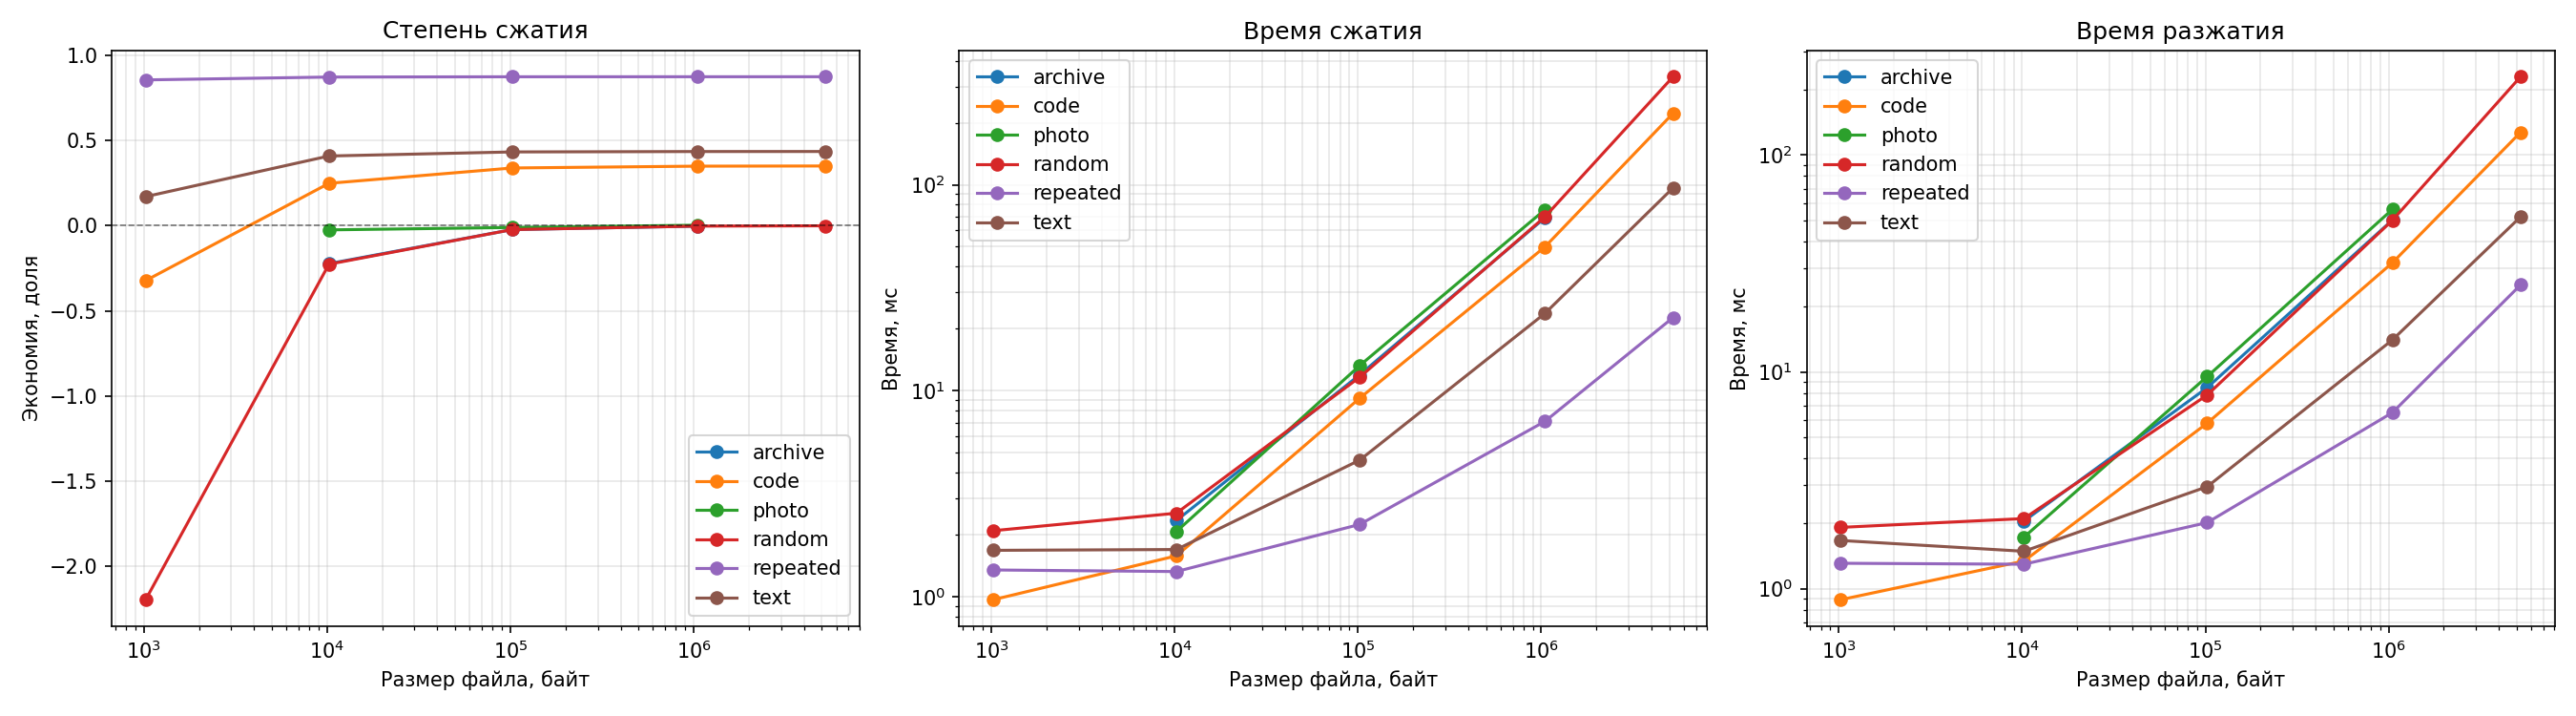
\includegraphics[width=\textwidth]{graphs.png}
    \caption{Зависимость степени сжатия и времени работы от размера файла}
    \label{fig:experiment}
\end{figure}

% ниже списком перечисляете то, что выносится как результат практики.
\subsection{Выводы из результатов эксперимента}

\begin{itemize}
    \item Эффективность сжатия определяется энтропией входных данных.
    Наибольшее сжатие достигается на однородных данных
    (\texttt{repeated}, 85.6--87.5\%): при одном уникальном символе
    код каждого байта занимает ровно один бит, что даёт восьмикратное
    уменьшение размера. Текстовые данные сжимаются на 41--44\%,
    исходный код~--- на 25--35\%. Процент сжатия слабо зависит
    от размера файла, начиная с~10~КБ.

    \item На уже сжатых (JPEG, ZIP) и случайных данных алгоритм
    неэффективен: размер файла, как правило, увеличивается на величину заголовка,
    зависящую от числа уникальных байтов.

    \item Маленькие файлы (менее~2--3~КБ) сжимаются неэффективно
    или увеличиваются в размере. В используемом формате заголовок
    содержит таблицу частот переменного размера: 8~байт на исходный
    размер, 2~байта на количество уникальных символов и по~9~байт
    на каждый уникальный символ (байт и восьмибайтовая частота).
    При полном алфавите из~256 символов заголовок занимает
    2314~байт, что превышает объём данных в~1~КБ.

    \item Время работы асимптотически линейно зависит от размера
    входного файла ($O(n)$): и сжатие, и разжатие выполняются за
    один проход по данным. На малых размерах относительный вклад
    фиксированных накладных расходов (открытие файла, инициализация
    структур) выше, поэтому график в логарифмических координатах
    идёт чуть менее круто, чем чистая линейная зависимость.

    \item Разжатие выполняется быстрее сжатия примерно в~1,2--1,9~раза на текстовых
    и случайных данных, на однородных данных времена сопоставимы.
    При сжатии дополнительно тратится время на построение дерева
    Хаффмана и генерацию кодов, тогда как при разжатии достаточно
    одного обхода дерева по битовому потоку.
    
    \item Случайные и уже сжатые данные обрабатываются медленнее,
    чем код, и намного медленнее, чем текст: из-за~256 уникальных
    символов средняя длина кода приближается к~8~битам, поэтому
    на каждый байт входа приходится записывать (или считывать)
    почти столько же бит, сколько занимал сам байт и экономии
    почти нет, а побитовых операций выполняется больше на тот же
    объём входных данных.
\end{itemize}

\section{Заключение}

В ходе выполнения работы получены следующие результаты:

\begin{itemize}
    \item изучена теория префиксных кодов и алгоритма Хаффмана;
    \item реализовано консольное приложение на C;
    \item настроены CI и статические анализаторы для Linux и Windows;
    \item написаны тесты, проверяющие работу архиватора;
    \item поставлены эксперименты, показавшие границы эффективной применимости алгоритма.
\end{itemize}

Репозиторий/ссылка на пуллреквест: \url{https://github.com/ada1ra/archiver_huffman/}.

Техническая документация: \url{https://github.com/ada1ra/archiver_huffman/blob/main/README.md}.

\section*{Список литературы}

\begin{enumerate}
    \item Huffman D.~A. A Method for the Construction of Minimum-Redundancy
    Codes // Proceedings of the IRE. — 1952. — Vol.~40, No.~9. — P.~1098--1101.

    \item SmnTin. huffman-archiver [Электронный ресурс]. — URL:
    \url{https://github.com/SmnTin/huffman-archiver}
    (дата обращения: 21.09.2026).

    \item MichaelDipperstein. huffman: Huffman code discussion and
    implementation [Электронный ресурс]. — URL:
    \url{https://github.com/MichaelDipperstein/huffman}
    (дата обращения: 21.09.2026).

    \item Connor Dye. C-Zip: File Compression and Decompression
    Application [Электронный ресурс]. — URL:
    \url{https://github.com/ConnorDye/C-Zip-File-Compression-and-Decompression-Application}
    (дата обращения: 21.09.2026).
\end{enumerate}

\end{document}
